\documentclass{beamer}
% Try the class options [notes], [notes=only], [trans], [handout],
% [red], [compress], [draft] and see what happens!

% \usepackage{definitions}
\usepackage[british]{babel}
\usepackage{color, soul}
\usepackage{tikz}

%% tikz tricks
% \tikzset{onslide/.code args={<#1>#2}{%
%   \only<#1>{\pgfkeysalso{#2}} 
% }}

\pdfinfo{
        /Title (cim)
        /Creator (LaTeX)
        /Producer (pdflatex)
        /Author (szerzo)
        /CreationDate (datum)
	/Subject (tema)
}


\mode<article> % only for the article version
{
  \usepackage{fullpage}
  \usepackage{hyperref}
}
\mode<presentation>
{
  \usetheme[left,width=0.65in,height=0.55in]{Kolozsvar}
  \setbeamercovered{transparent}
  \setbeamertemplate{navigation symbols}{}
  \setbeamertemplate{footline}%
     {\vspace*{-1.4em}\hspace*{0.66in}\textbf{\insertframenumber/\inserttotalframenumber}\newline\vspace*{0.4em}}
		\setbeamerfont{block title}{size=\larger} % RELSIZE -- html-sizes 
		\usefonttheme{professionalfonts}
		\setbeamercolor{math text}{fg=green!30!red!30!brown}
		\setbeamercolor{normal text in math text}{parent=math text}
}

\setbeamercovered{dynamic}

% The following info should normally be given in you main file:
\title[IoT in 5G Era]{IoT in 5G Era}

%
\author{Hunor Ördög, Norbert-Raymond Pap, István-Lehel Balázs}
%
\institute[UBB Cluj-Napoca]{
  Department of Mathematics and Informatics\\
  Babe{\c{s}}--Bolyai University, Cluj-Napoca}
%
\date{2024 December}


\begin{document}

\frame{\maketitle}

\mode<presentation>
{
  % \begin{frame}
  %   \frametitle{Talk structure}
  % \tableofcontents
  % \end{frame} 

  % \AtBeginSection[]
  {
      \begin{frame}<beamer>{Contents}
        % \tableofcontents[currentsection,currentsubsection,hideothersubsections]
        \tableofcontents
      \end{frame}
    }
}

%%%%%%%%%%%%%%%%%%%%%%%%%%%%%%%%%%%%%%%%%%%%%%%%%%%%%%%%%%%%%%%%%%%%%%

% \section[Brand changes - 28 oct 2024]{Brand changes - 28 oct 2024}

% \begin{frame}{Brand changes - 28 oct 2024}
  % \hspace*{2.3em}
  % \includegraphics[scale=0.25]{fig/sonar-rebrand-1.jpg}
% \end{frame}


% \section[Introduction]{Introduction}

% \begin{frame}{What is Sonar?}
%   \begin{itemize}
%     \item Tool for \textbf{code quality} and \textbf{security} throughout the development lifecycle.
%     \vspace*{0.75em}
%     \item Catch \textbf{bugs}, \textbf{vulnerabilities}, and \textbf{design issues} 
%     (Duplicated code, Large methods, Inconsistent naming).
%     \vspace*{0.75em}
%     \item Improve \textbf{maintainability}, \textbf{readability}, and \textbf{security}.
%   \end{itemize}
% \end{frame}

% Begin Hunor
\section[Introduction]{Introduction}

\begin{frame}{5G and IoT: A Perfect Match}
  \begin{itemize}
      \item Rapid expansion of IoT and 5G.
      \vspace*{0.7em}
      \item 5G's role in supporting IoT's diverse applications.
      \vspace*{0.7em}
      \item Enhanced capabilities like low latency, high reliability, and massive device connectivity.
      \vspace*{0.7em}
      \item The combination of 5G and edge computing supports time-critical IoT applications.
  \end{itemize}
\end{frame}

\begin{frame}{Phases of 5G implementation}
  \begin{itemize}
      \item 3GPP Release 15 2018, first phase of 5G standardization.
      \vspace*{0.5em}
      \item 3GPP Release 16 2020, second phase, enhances capabilities and supports ultra reliable low-latence communication.
      \vspace*{0.5em}
      \item 3GPP Release 17 2022, RedCap, NTN (Non-Terrestrial Networks), 5G New Radio (NR) - standard for the air interface of the 5G network.
  \end{itemize}
\end{frame}

\begin{frame}{5G's Vision for Connectivity}
  \begin{itemize}
      \item \textbf{Peak Data Rate:} 20 Gbps - 10x 4G.
      \vspace*{0.4em}
      \item \textbf{Latency:} Reduced to 1 ms 10x improvement.
      \vspace*{0.4em}
      \item \textbf{Connection Density:} 1,000,000 devices/km$^2$.
      \vspace*{0.4em}
      \item \textbf{Energy Efficiency:} 100-fold improvement.
      \vspace*{0.4em}
      \item \textbf{Mobility:} Supports speeds $>$ 120 km/h.
  \end{itemize}
\end{frame}

\begin{frame}{5G Frequency Ranges}
  \begin{itemize}
      \item \textbf{Frequency Range 1 (FR1):} Sub-6 GHz bands.
      \vspace*{0.75em}
      \item \textbf{Frequency Range 2 (FR2):} 24–100 GHz (also called millimeter wave).
  \end{itemize}
\end{frame}

% \begin{frame}{5G's Core Application Clusters}
%   \begin{itemize}
%       \item \textbf{eMBB:} Enhanced Mobile Broadband (e.g., HD video streaming).
%       \vspace*{0.5em}
%       \item \textbf{mMTC:} Massive Machine Type Communications (e.g., IoT sensors).
%       \vspace*{0.5em}
%       \item \textbf{URLLC:} Ultra-Reliable Low-Latency Communications (e.g., autonomous vehicles).
%   \end{itemize}
% \end{frame}

% \begin{frame}{Evolution of Cellular Networks}
%   \begin{itemize}
%       \item Latency: 10 ms (4G) vs. 1 ms (5G).
%       \item Peak Data Rate: 1 Gbps (4G) vs. 20 Gbps (5G).
%       \item Connection Density: 100x improvement.
%       \item Energy Efficiency: 100x improvement.
%   \end{itemize}
% \end{frame}

\begin{frame}{5G vision}
  \hspace*{0.4em}
  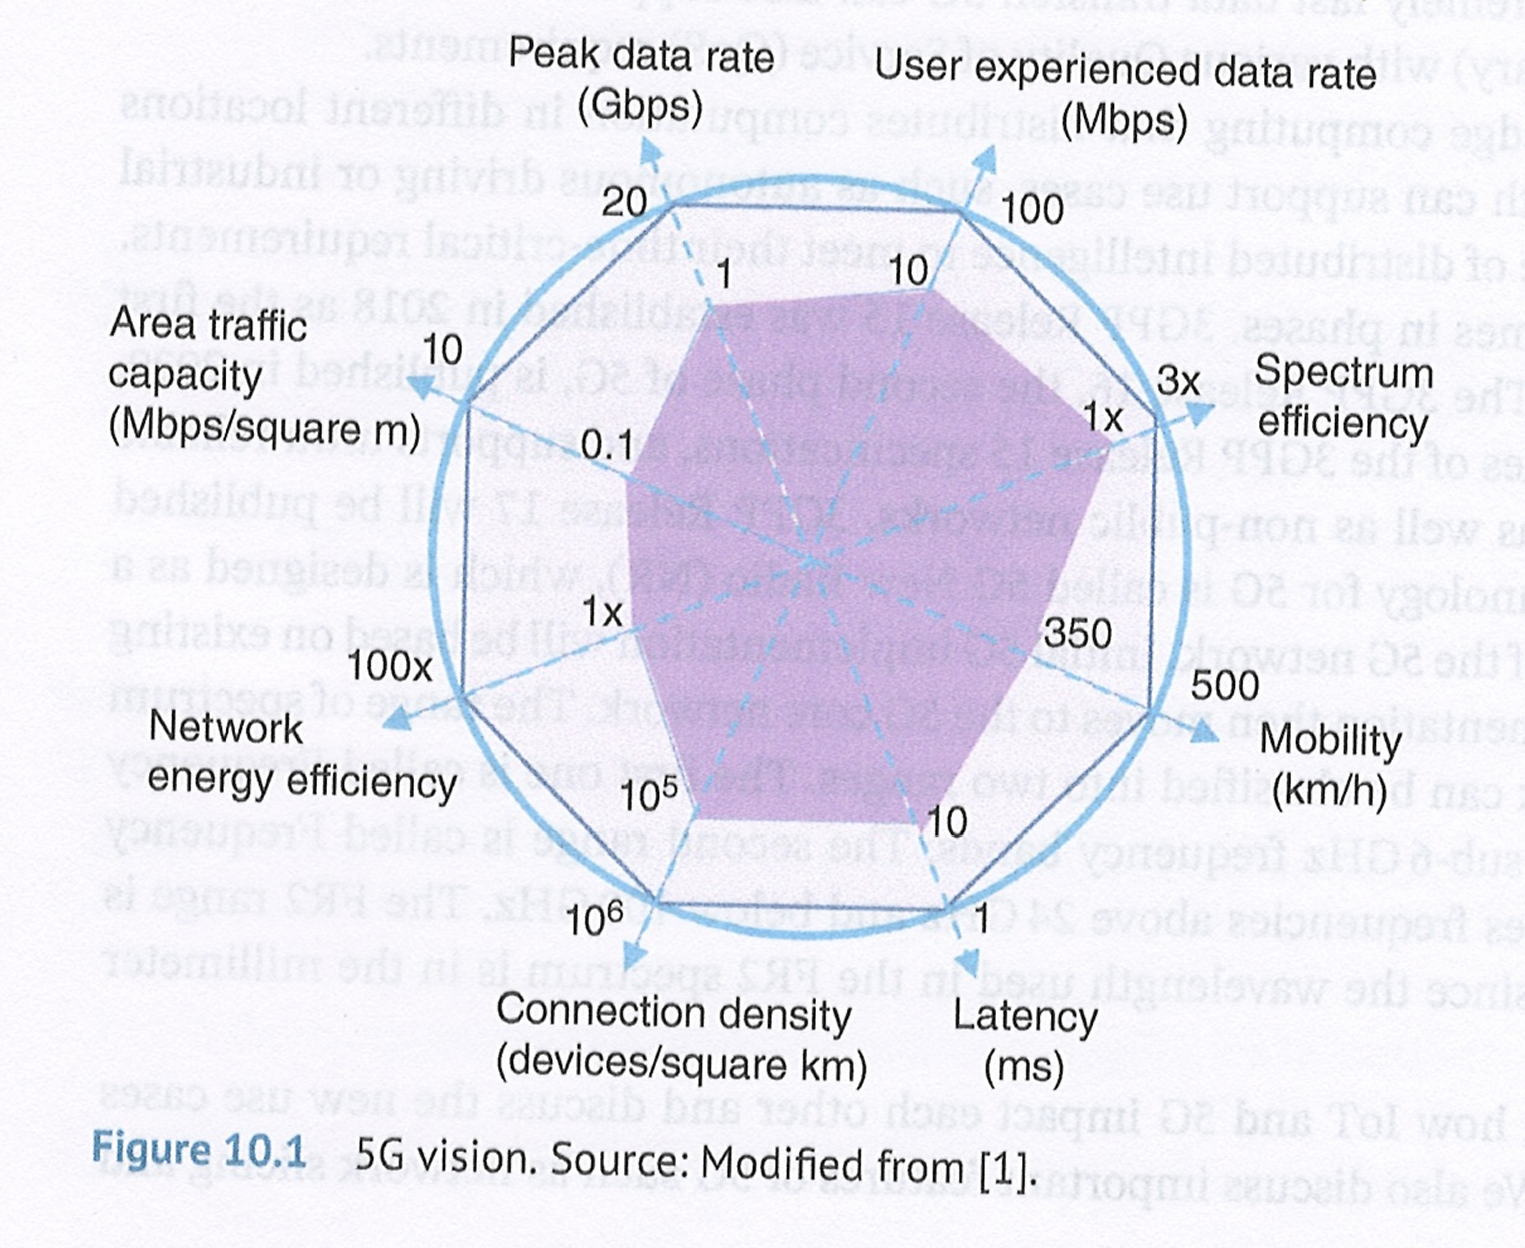
\includegraphics[scale=0.5]{fig/5g-vision-fig-10-1.png}
\end{frame}

% \begin{frame}{Real-World Applications of 5G IoT}
%   \begin{itemize}
%       \item \textbf{Smart cities:} Connected utilities and infrastructure.
%       \item \textbf{Autonomous vehicles:} Real-time navigation.
%       \item \textbf{Industrial IoT:} Factory automation and robotics.
%   \end{itemize}
% \end{frame}

% End Hunor

\section[5G Main Application Areas]{5G Main Application Areas}

\begin{frame}{5G Main Application Areas}
  \vspace*{1.6em}
  \begin{itemize}
    \item Mobile Broadband (eMBB)
    \vspace*{0.75em}
    \item massive Machine Type Communications (mMTC)
    \vspace*{0.75em}
    \item Ultra Reliable and Low-Latency Communications (URLLC)
  \end{itemize}
\end{frame}

\begin{frame}{Overview of 5G application areas}
  \hspace*{0.6em}
  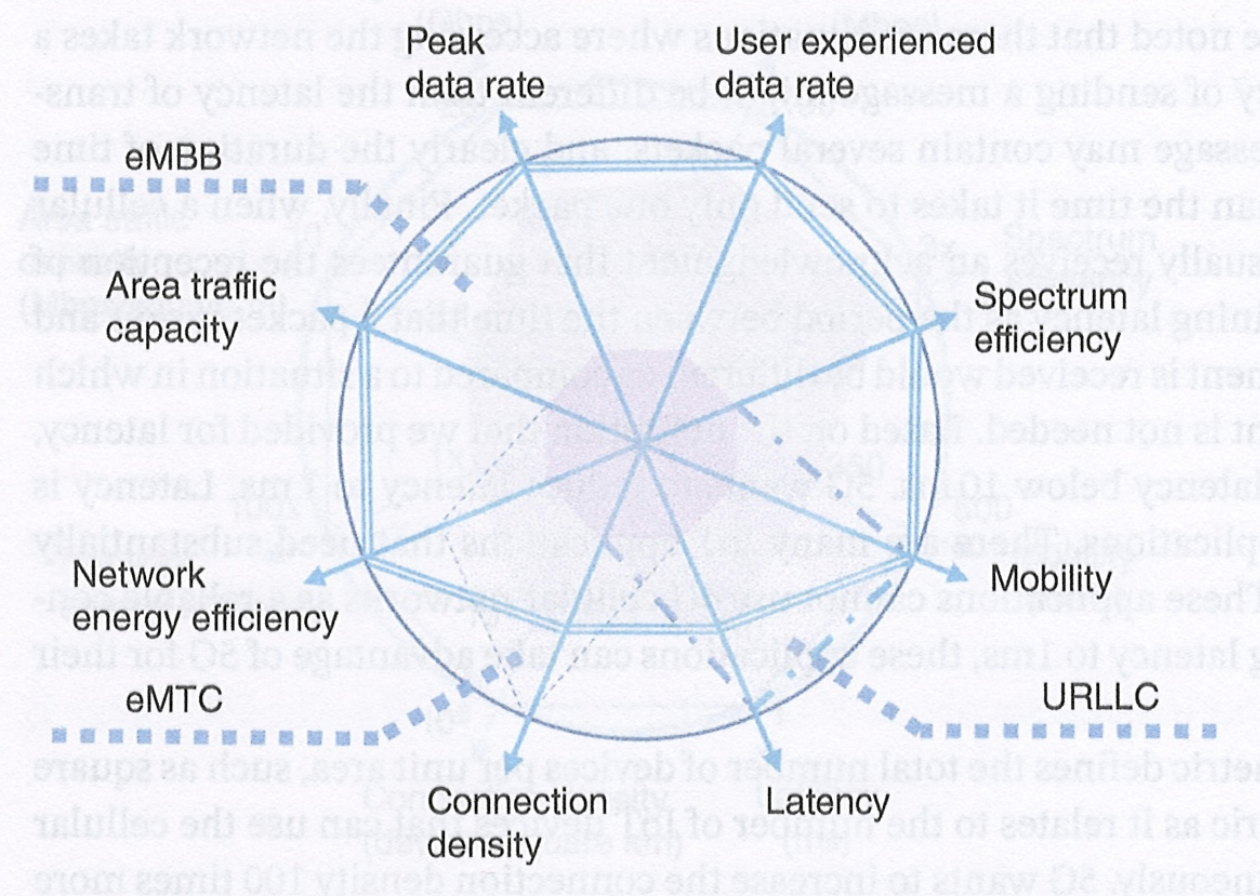
\includegraphics[scale=0.45]{fig/5g_application_areas.png}
\end{frame}

\begin{frame}{Mobile Broadband (eMBB)}
  \vspace*{1.6em}
  \begin{itemize}
    \item delivery of voice and high-speed data
    \vspace*{0.75em}
    \item larger system capacity, data throughput, more efficient than 4G
    \vspace*{0.75em}
    \item Example: supports high-definition IoT cameras used for surveilliance
  \end{itemize}
\end{frame}

\begin{frame}{massive Machine Type Communications (mMTC)}
  \vspace*{1.6em}
  \begin{itemize}
    \item machine-to-machine type communications
    \vspace*{0.75em}
    \item supports large number of IoT devices with diverse range of requirements in terms of bandwidth
  \end{itemize}
\end{frame}

\begin{frame}{Ultra Reliable and Low-Latency Communications (URLLC)}
  \vspace*{1.6em}
  \begin{itemize}
    \item very important part of 5G, vital for ultra-reliable and critical IoT systems
    \vspace*{0.75em}
    \item supports self-driving cars or enhanced factory automation applications
  \end{itemize}
\end{frame}

\section[5G Implementations and Features]{5G Implementations and Features}

\begin{frame}{Standalone and non-stanadlone 5G Network}
  \vspace*{1.6em}
  \begin{itemize}
    \item 5G Network Components
    \begin{itemize}
        \item 5G RAN: Handles radio technologies and base stations.
        \item 5G Core: Manages functions such as authentication, signaling, paging, mobility, and security.
    \end{itemize}
    \item Deployment Types
    \begin{itemize}
        \item Non-Standalone (NSA)Combines 5G RAN for data communication with the 4G core for signaling and control.
        \item Standalone (SA): Both data and signal planes operate using the 5G core.
    \end{itemize}
    \item Most 5G networks today use the NSA deployment model.
  \end{itemize}
\end{frame}

\begin{frame}{Standalone and non-stanadlone 5G Network}
  \hspace*{0.6em}
  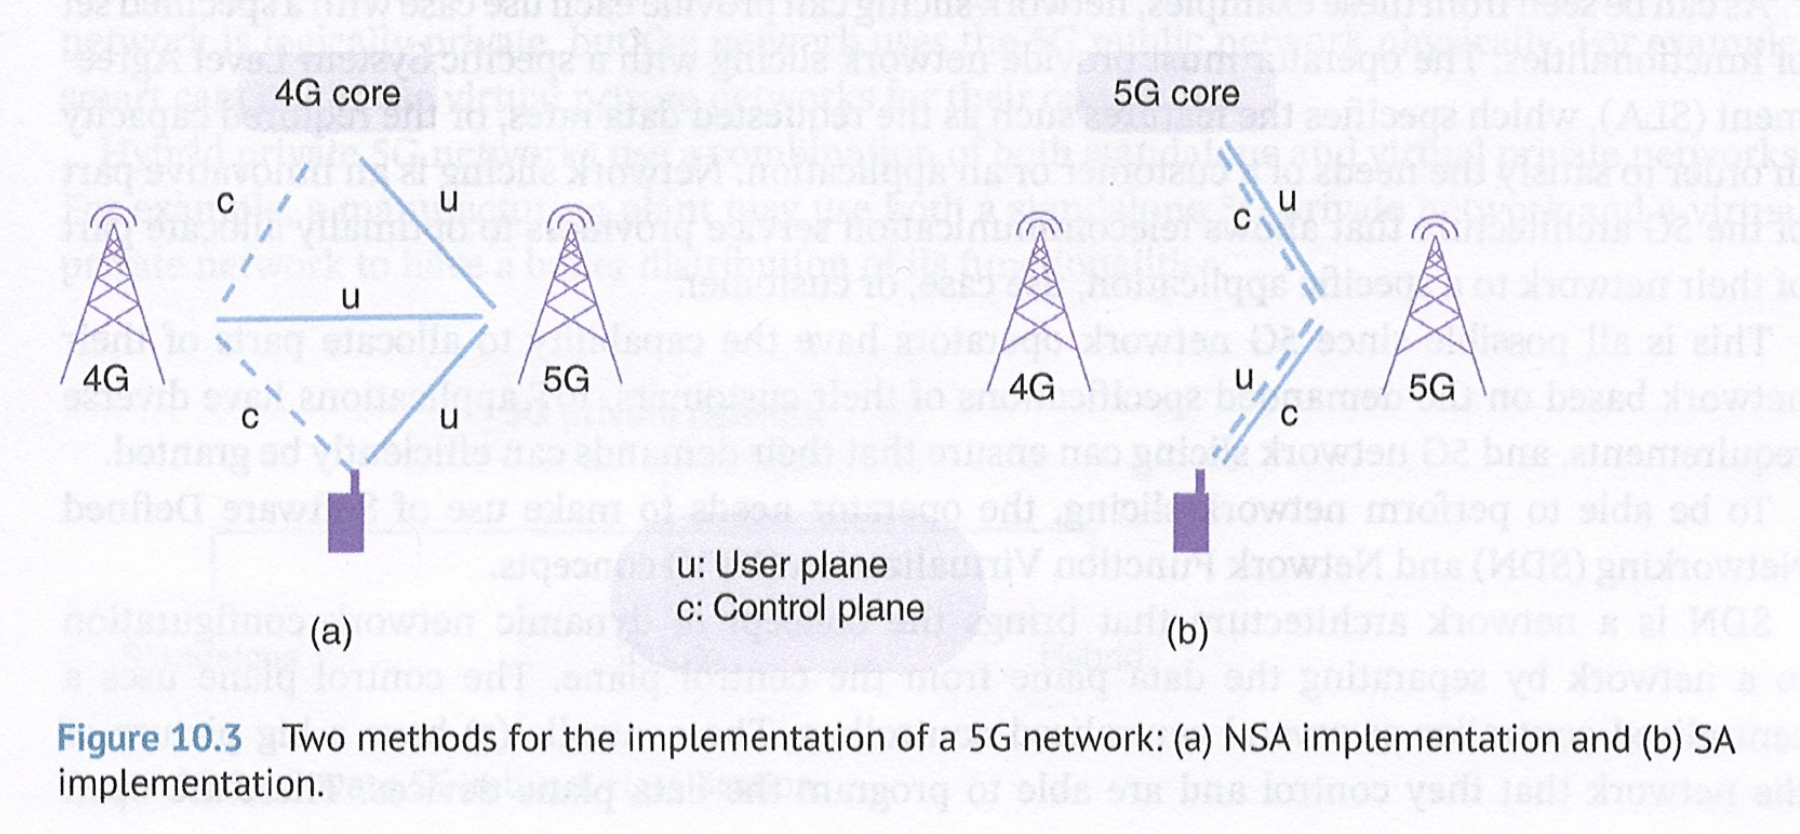
\includegraphics[scale=0.33]{fig/standalone_and_not.png}
\end{frame}

\begin{frame}{5G Network Slicing}
  \begin{itemize}
    \item Virtualizes the 5G network into multiple logical slices, each tailored to specific use cases, businesses, or customers.
    \item Slices: eMBB, URLLC, mMTC
    \item Slicing types
    \begin{itemize}
        \item Single Slicing: One slice per specific use case.
        \item Bundle Slicing: Combines multiple slices for complex needs.
    \end{itemize}
    \item Examples
    \begin{itemize}
        \item Logistics: Low-latency, mobility-enabled slice.
        \item Smart Cities: High-availability slices for fire alarms.
        \item Stadiums: High-throughput eMBB slice for visitors.
        \item Manufacturing: Reliable, low-latency URLLC slice.
    \end{itemize}
    \item Relies on Software-Defined Networking (SDN) and Network Function Virtualization (NFV) to dynamically configure and optimize the network.
  \end{itemize}
\end{frame}

\begin{frame}{Overview - 5G Slicing}
  \hspace*{0.6em}
  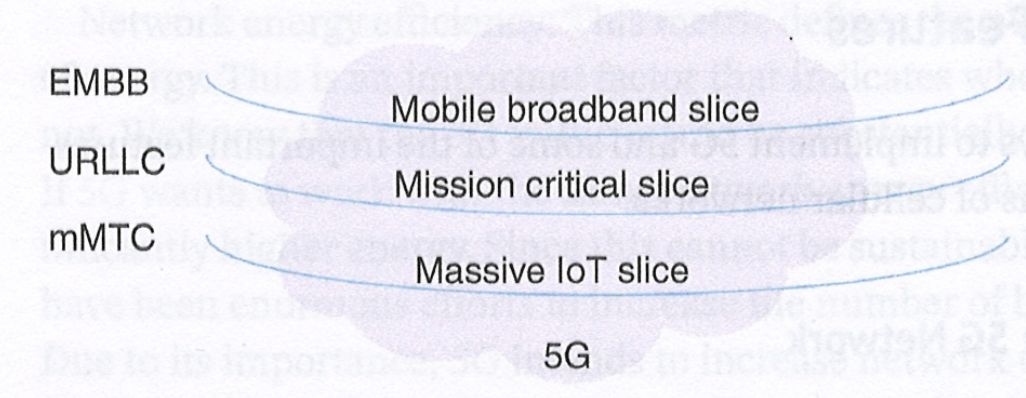
\includegraphics[scale=0.6]{fig/5g_slices.png}
\end{frame}

\section[Private 5G Network]{Private 5G Network}

\begin{frame}{Private 5G Network Classification}
  \hspace*{0.6em}
  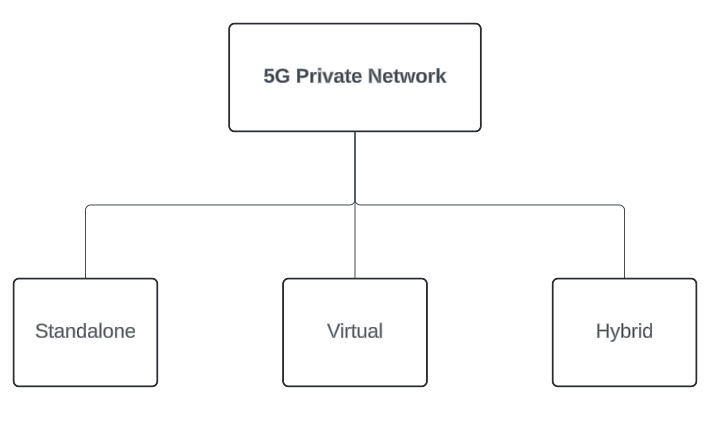
\includegraphics[scale=0.6]{fig/5gprivate.png}
\end{frame}


\begin{frame}{Standalone Private Network}
  \vspace*{1.6em}
  \begin{itemize}
    \item Purchased from an operator.
    \vspace*{0.75em}
    \item Mantained by customer.
    \vspace*{0.75em}
    \item Example: Airport - isolated network deployed physically at the airport's vicinity.
  \end{itemize}
\end{frame}

\begin{frame}{Virtual Private Network}
  \vspace*{1.6em}
  \begin{itemize}
    \item Virtualization on public 5G networks.
    \vspace*{0.75em}
    \item Logically private, but physically using the public network.
    \vspace*{0.75em}
    \item Example: Smart cars - virtual private network for operations.
  \end{itemize}
\end{frame}

\begin{frame}{Hybrid Private Network}
  \vspace*{1.6em}
  \begin{itemize}
    \item Combination of standalone and virtual.
    \vspace*{0.75em}
    \item Example: Manufacturing plant - enabling better distribution of functionalities along with broad coverage, high capacity, and cost-efficiency.
  \end{itemize}
\end{frame}

\section[Network exposure]{Network exposure}


\begin{frame}{What is Network Exposure in 5G?}
  \vspace*{1.6em}
  \begin{itemize}
    \item Allow customers and partners to access network services and capabilities via  easy-to-use APIs.
    \item Enables customers and partners to use network resources based on the needs of their applications.
    \item Crucial for IoT applications.
    \item Access is controlled by strict policies to ensure data integrity and protection.
  \end{itemize}
\end{frame}


\begin{frame}{Ericson's IoT experiment}
  \vspace*{1.3em}
  \begin{itemize}
    \item A remote controlled drone connected to 5G network is used to inspect a tower.
    \item The application uses APIs to trigger an exposure server on a 5G core network.
    \item API\#1 triggers exposure server to connect to the drone, authenticate, send it towards the tower.
    \item Inspection camera doesn't need to send high-quality video. 
  \end{itemize}
\end{frame}

\begin{frame}{Ericson's IoT experiment}
  \vspace*{1.6em}
  \begin{itemize}
    \item When the drone gets closer the application sends to API\#2 to increase bandwidth.
    \item Before reaching the tower the application sends to API\#3 to add URLLC slice for remote control, increase the quality of video.
    \item After the control the application sends to API\#4 to erase URLLC slice and lower the quality.
  \end{itemize}
\end{frame}

\begin{frame}{Experiment summary}
  \hspace*{0.4em}
  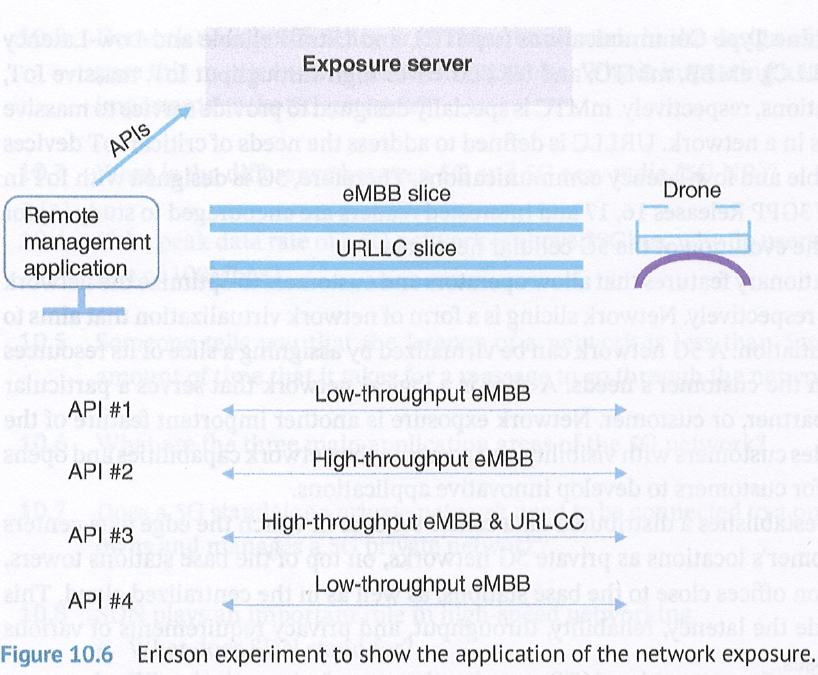
\includegraphics[scale=0.52]{fig/exposure-exp.png}
\end{frame}


\section[Fixed Wireless Access]{Fixed Wireless Access}


\begin{frame}{Fixed Wireless Access (FWA)}
  \vspace*{1.6em}
  \begin{itemize}
    \item Some locations don't have acces to wired internet connection.
    \vspace*{0.75em}
    \item 5G FWA can be used to provide internet access cost-effectively.
    \vspace*{0.75em}
    \item This way IoT devices can also get good internet access on remote places.
  \end{itemize}
\end{frame}


\section[Summary]{Summary}


\begin{frame}{Summary}
  \begin{itemize}
    \item enhanced Mobile BroadBand (eMBB).
    \vspace*{0.75em}
    \item massive Machine Type Communications (mMTC).
    \vspace*{0.75em}
    \item Ultra-Reliable and Low-Latency Communications (URLLC).
    \vspace*{0.75em}
    \item Network Slicing, Network Virtualization.
    \vspace*{0.75em}
    \item Private Networks, FWA.
  \end{itemize}
\end{frame}



\section[Exercises]{Exercises}


\begin{frame}{Exercises}
  \textbf{Question:} Compare 4G and 5G networks based on latency, speed, capacity, bandwidth and energy consumption.
\end{frame}

\begin{frame}{Exercises}
  \textbf{4G Network:}
  \begin{itemize}
    \item Latency: 30-50 ms
    \item Speeds: 1 Gbps (stationary), 100 Mbps (mobile)
    \item Capacity: 2,000 devices/km\(^2\)
    \item Bandwidth: Sub-6 GHz, limited in dense areas
    \item Energy: Higher per bit
  \end{itemize}
  \vspace{0.5cm}
  \textbf{5G Network:}
  \begin{itemize}
    \item Latency: As low as 1 ms
    \item Speeds: Up to 20 Gbps
    \item Capacity: 1 million devices/km\(^2\)
    \item Bandwidth: Sub-6 GHz + mmWave (24 GHz+)
    \item Energy: Lower per bit
  \end{itemize}
\end{frame}

\begin{frame}{Exercises}
  \textbf{Question:} 5G Supports 24-100Ghz frequency range, called FR2. What is the rande of wavelengths of FR2?
\end{frame}


\begin{frame}{Exercises}
  \textbf{Question:} 5G Supports 24-100Ghz frequency range, called FR2. What is the rande of wavelengths of FR2?
  \vspace*{0.75em}
  \begin{itemize}
    \item \textbf{Formula:} \(wavelength = \frac{c}{f}\), where \(c = 3 \times 10^8 \, \text{m/s}\)
    \item \textbf{For 24 GHz:}
    \[
    f = 24 \, \text{GHz} = 24 \times 10^9 \, \text{Hz}
    \]
    \[
      wavelength = \frac{3 \times 10^8 \, \text{m/s}}{24 \times 10^9 \, \text{Hz}} = 0.0125 \, \text{m} = 1.25 \, \text{cm}
    \]
    \item \textbf{For 100 GHz:}
    \[
    f = 100 \, \text{GHz} = 100 \times 10^9 \, \text{Hz}
    \]
    \[
      wavelength = \frac{3 \times 10^8 \, \text{m/s}}{100 \times 10^9 \, \text{Hz}} = 0.003 \, \text{m} = 3 \, \text{mm}
    \]
  \end{itemize}
\end{frame}

\begin{frame}{Exercises}
  \textbf{Question:} If the peak rate of 5G network is above 20Gbps, why do users only experience a data rate of 100Mbps?
\end{frame}


\begin{frame}{Exercises}
  \textbf{Question:} If the peak rate of 5G network is above 20Gbps, why do users only experience a data rate of 100Mbps?
  \vspace*{0.75em}
  \begin{itemize}
    \item It is not possible for the network to allow the user to transmit continuously using max number of possible data rate at all times.
    \item It has to share the resources between all the users in a cell.
    \item The data rate a user can experience depends on the location of the device in the cell, number of devices in the cell, their traffic pattern.
  \end{itemize}
\end{frame}


\begin{frame}{Exercises}
  \textbf{Question:} Does a 5G standalone private network need to be connected to a public 5G network? Who owns and manages it?
\end{frame}

\begin{frame}{Exercises}
  \textbf{Question:} Does a 5G standalone private network need to be connected to a public 5G network? Who owns and manages it?
  \vspace*{0.75em}
  \begin{itemize}
    \item No, it is isolated from the public network. 
    \item Standalone private networks are the ones purchased from the provider, and managed by the customer.
  \end{itemize}
\end{frame}


\end{document}
